% Dokumentanklasse: a4paper, 14pt
% Beschreibung:     Dokumentenformat
% Option:           extraarticle - ?
\documentclass[12pt]{article}

% Packet:           xcolor
% Beschreibung:     Define own color schemas
% Option:
% Restriktion:      Muss vor Paket hyperref geladen werden. Ansonsten werden die Farben der Links nicht genutzt.
\usepackage{xcolor}

% Definiere Farben
\definecolor{blue}{HTML}{5E7FB8}
\definecolor{brown}{HTML}{BA9D5E}
\definecolor{green}{HTML}{79B960}
\definecolor{grey}{HTML}{7C7C7C}
\definecolor{light-grey}{HTML}{D5D5D5}
\definecolor{orange}{HTML}{FF7F00}
\definecolor{red}{HTML}{B80A0A}
\definecolor{violet}{HTML}{B688CB}
\definecolor{white}{HTML}{FFFFFF}
\definecolor{yellow}{HTML}{E2E66C}

% Paket:            setspace
% Beschreibung:     Setz über die optionen den Zeilenabstand
% Optionen:         Möglicher Zeilenabstand
%                   singlespacing = 1,0
%                   onehalfspacing = 1,5
%                   doublespacing = 2,0
% Restriktion:      Muss vor Paket hyperref geladen werden. Ansonsten funktioniert das Paket nicht.
\usepackage[onehalfspacing]{setspace}


% ###########################################################################################################################

% Paket:            appendix
% Beschreibung:     Das Paket dient dazu, ausschließlich das Thema einer Überschrift in das Inhaltsverzeichnis zu überführen
% Option:           appendix - Überführt die Überschriften des Anhangs richtig ins das Inhaltsverzeichnis
\usepackage[titletoc]{appendix}

% Paket:            ansmath
% Beschreibung:     Zum darstellen von mathematischen Formeln
\usepackage{amsmath}

% Paket:            bebel
% Beschreibung:     Stellt das Literatur-, Abbilungs-, Tabellenverzeichnis auf eine beliebige Sprache
% Option:           ngerman
\usepackage[ngerman]{babel}

% Paket:            biblatex
% Beschreibung:     Ermöglicht es, ein Literaturverzeichnis zu führen
% Option:
\usepackage[
  style=authoryear-icomp,    % Zitierstil (https://de.overleaf.com/learn/latex/Biblatex_bibliography_styles)
  isbn=false,                % ISBN nicht anzeigen, gleiches geht mit nahezu allen anderen Feldern
  pagetracker=true,          % ebd. bei wiederholten Angaben (false=ausgeschaltet, page=Seite, spread=Doppelseite, true=automatisch)
  maxbibnames=50,            % maximale Namen, die im Literaturverzeichnis angezeigt werden
  maxcitenames=3,            % maximale Namen, die im Text angezeigt werden, ab 4 wird u.a. nach den ersten Autor angezeigt
  autocite=inline,           % regelt Aussehen für \autocite (inline=\parancite)
  block=space,               % kleiner horizontaler Platz zwischen den Feldern
  backref=true,              % Seiten anzeigen, auf denen die Referenz vorkommt
  backend=biber,
  backrefstyle=three+,       % fasst Seiten zusammen, z.B. S. 2f, 6ff, 7-10
  date=short,                % Datumsformatbackend=biber
]{biblatex}
\setlength{\bibitemsep}{1em}     % Abstand zwischen den Literaturangaben
\setlength{\bibhang}{2em}        % Einzug nach jeweils erster Zeile
\addbibresource{referenzen//bibliothek.bib}

% Paket:            caption
% Beschreibung:     Bietet eine große Auswahl an Gestaltungsmöglichkeiten bezüglich der Beschriftung von Bildern und Tabellen.
\usepackage{caption}

% Paket:            colortbl
% Beschreibung:     Ermöglicht Tabellen, Spalten oder Zellen farbig zu gestalten.
% Befehle:          \columncolor
% Dokumentation:    http://texdoc.net/texmf-dist/doc/latex/colortbl/colortbl.pdf
\usepackage{colortbl}

% Paket:            booktabs
% Beschreibung:     Das Hauptaugenmerk von booktabs liegt dabei auf der Gestaltung der horizontalen Linien innerhalb einer Tabelle.
%                   Was unter anderem daran liegt, dass der Autor des Paketes Simon Fear mehrere Regeln bzw. Empfehlungen für die
%                   Erstellung/Gestaltung einer Tabelle gibt. Aufgrund der ersten zwei Regeln:
%                   1) Verwende nie und nimmer vertikale Linien.
%                   2) Verwende keine doppelten Linien.
% Dokumentation:    https://www.namsu.de/Extra/pakete/Booktabs.html
\usepackage{booktabs}

% Paket:            courier
% Beschreibung:     Lädt das Paket courier für Schriftarten mit fester Breite.
% Befehle:          \ttfamily     Aktiviert Courier füt Tabellen bzw. generelle begin-Blöcke
\usepackage{courier}

% Packet:           csquotes
% Beschreibung:     Muss nach babel, polyglossia, biblatex und inputec geladen werden
% Options:
%   autostyle=true  - Diese Anweisung passt das Zitatdesign so an, dass es zur momentan im Dokument verwendeten Sprache passt
%   autostyle=once  - Ändert das Zitatdesign einmalig, sodass es zur Grundsprache des Dokumentes passt.
%   autostyle=try   - Verhalten sich, sollte multilinguale Unterstützung vorhanden sein, wie true und once, doch werden sie,
%                     für den Fall, dass dies nicht möglich wäre, keine Warnungen erzeugen. (D. h. falls weder babel noch
%                     polyglossia geladen wurden). Die Kurzformautostyleist äquivalent zu autostyle=true
% Dokumentation:    http://mirrors.ibiblio.org/CTAN/info/translations/csquotes/de/csquotes-DE.pdf
\usepackage[autostyle=true]{csquotes}

% Paket:            enumitem
% Beschreibung:     Zeilenabstände bei Aufzählungen definieren
% Option:
\usepackage{enumitem}

% Paket:            eurosym
% Beschreibung:     Bildet das Euro-Zeichen in unterschiedlichen Varianten ab
% Option:
\usepackage{eurosym}

% Paket:            fancyhdr
% Beschreibung:     Ermöglich ein generelles Seitenlayout ein zu stellen mit Kopf und Fußzeile.
\usepackage{fancyhdr}

% Paket:            float
% Beschreibung:     Zum Ausrichten von Tabellen und Spalten bzw. deren Zentrierung
% Option:
% Restriktion:      Muss von Paket hyperref geladen werden. Ansonsten funktioniert das Paket nicht.
\usepackage{float}

% Packet:           framemethod
% Beschreibung:
% Option:
\usepackage[framemethod=tikz]{mdframed}
\mdtheorem[
  linecolor=red,
  frametitlefont=\sffamily\bfseries\color{white},
  frametitlebackgroundcolor=red,
]{warn-popup}{Warnung}[subsection]

\mdtheorem[
  linecolor=orange,
  frametitlefont=\sffamily\bfseries\color{white},
  frametitlebackgroundcolor=orange,
]{info-popup}{Information}[subsection]

\mdtheorem[
  linecolor=green,
  frametitlefont=\sffamily\bfseries\color{white},
  frametitlebackgroundcolor=green,
]{example-popup}{Beispiel}

% Paket:            footmisc
% Beschreibung:     Das footmisc Paket liefert viele Möglichkeiten, wie Fußnoten in Dokumenten dargestellt werden können.
% Option:
% Dokumentation:    http://mirror.utexas.edu/ctan/info/translations/footmisc/de/footmiscDE.pdf
\usepackage[bottom]{footmisc}

% Paket:            geometry
% Beschreibung:     A4 Seitenabstände
% Option:
\usepackage{geometry}
\geometry{
%  a4paper,           % Papierformat (wird auch über die Dokumentenklasse definiert)
  top=2.5cm,          % Abstand Kopfseite   (Zwischen Kopfseite und Inhalt)
  bottom=2cm,         % Abstand Fußseite    (Zwischen Fußseite und Inhalt)
  left=2.5cm,         % Abstand Linkeseite  (Zwischen Linkerseite und Inhalt)
  right=2.5cm,        % Abstand Rechteseite (Zwischen Recherseite und Inhalt)
%  width=              %                    textwidth (+marginsep +marinparwidth)
%  textwidth=15cm,     % Textbreite
%  marginparsep=1cm,   % Randnotiztrennng
%  marginparwidth=10cm,% Randnotizbreite
%  height=             %                    textheight (+headheight +headsep + footskip)
%  textheight=        % Texthöhe
  headheight=1cm,     % Kopfhöhe
  headsep=0.5cm,      % Kopftrennung        (Größe zwischen Kopfzeile und Inhalt)
  footskip=1cm,       % Fußzeilenhöhe
}

% Paket:            graphicx
% Beschreibung:     Einbinden von Bildern
% Option:
\usepackage{graphicx}

% Packet:           Hyperref
% Beschreibung:     Importiert hyperref um Querverweise mittels \hyperref zu erzeugen.
% Dokumentation:    https://www.namsu.de/Extra/pakete/Hyperref.html
\usepackage{hyperref}
\hypersetup{
  colorlinks=false,                 % hyperlinks are coloured
  citecolor=green,                  % color for cite links, only visible if colorlinks=true
  linkcolor=red,                    % color for page links, only visible if colorlinks=true
  urlcolor=orange,                  % color for url links, only visible if colorlinks=true
  citebordercolor=green,            % color for citeborder, only visible if colorlinks=true
  urlbordercolor=orange,            % color for url links, only visible if colorlinks=true
  linkbordercolor=red,              % color for page links, only visible if colorlinks=true
  pdfborderstyle={/S/U/W 1},        % border style will be underline of width 1pt
  pdftitle={Data-Warehouse},
  pdfauthor={Markus Pesch},
  pdfsubject={Zusammenfassung},
  pdfkeywords={},
  pdfcreator={pdflatex},
  pdfproducer={LaTeX with hyperref}
}

% Paket:            glossaries
% Beschreibung:     Das Paket glossaries muss nach dem Paket hyperref geladen werden
% Dokumentation:    http://ftp.gwdg.de/pub/ctan/macros/latex/contrib/glossaries/glossaries-user.pdf
% Option/en:
%   acronyms        - This is equivalent to acronym=true and may be used in the document class option list.
%   section         - This is a key=value option. Its value should be the name of a sectional unit (e.g. chapter).
%                     This will make the glossaries appear in the named sectional unit, otherwise each glossary will
%                     appear in a chapter, if chapters exist, otherwise in a section. Unnumbered sectional units will
%                     be used by default.
%   toc             - Add the glossaries to the table of contents.
\usepackage[toc,acronyms]{glossaries}
\makeglossaries
\include{referenzen/glossar}

% Paket:            utf8
% Beschreibung:     Stellt Umlaute richtig dar
% Option:           inputenc - Erlaubt die Darstellung der gleichen Zeichen (Character) wie sie in stdin überliefert werden
\usepackage[utf8]{inputenc}

% Paket:            lipsum
% Beschreibung:
% Option:
\usepackage{lipsum}

% Paket:            makeindex
% Beschreibung:     Ermöglicht das Indexieren von Wörter und den Befehl \printindex um den Index auszugeben
\usepackage{makeidx}
\makeindex

% Packet:           Minted
% Beschreibung:     Dient zum highlining von Quellcode wie beispielsweise Java, Bash oder Python.
% Option/en:
%   autogobble:       Leerzeichen zwischen linken Rand und Sourcecode einrücken bzw. weg schneiden.
%   breaklines:       Automatische Zeilenumbrüche
%   cache:            de- oder aktiviert den cache um Sourcecode zwischen zu speichern und so das PDF schneller zu erzeugen
%   cachedir:         Definiert den Pfad zum cache, an dem minted seine Daten zwischen speichern kann
%   fontfamily:       Die Schriftart die benutzt werden soll. tt, courier und helvetica sind vordefiniert.
%   fontsize:         Die Schriftgröße die benutzt werden soll. Beispielsweise fontsize=\footnotesize
%   linenos:          Zeilennummern
%   keywordcase:      Änderung der Buchstaben. Takes lower, upper, or capitalize.
%   showspaces:       Blendet Leerzeichen ein
\usepackage[cache=true]{minted}

% usemintedstyle
% Gebe 'pygmentize -L styles' im Terminal ein um alle verfügbaren styles anzuzeigen.
\usemintedstyle{tango}

% newminted
% Definiere neue aliase um einmalig ein highlighting pro Sprache zu deklarieren
% \newminted{<makroname>}{optionen} ist verfügbar unter "<makroname>code"
\newminted{awk}{autogobble=true, breaklines=true, linenos=true}
\newminted{json}{autogobble=true, breaklines=true, linenos=true}
\newminted{julia}{autogobble=true, breaklines=true, linenos=true}
\newminted{r}{autogobble=true, breaklines=true, linenos=true}
\newminted{sql}{autogobble=true, breaklines=true, linenos=true, keywordcase=upper}
\newminted{xml}{autogobble=true, breaklines=true, linenos=true}

% newmintedfile
% Definiere neue Makros um automatisch Sourcecode aus Dateien zu highlighten.
% \makroname{Dateipfad}
\newmintedfile[inputawk]{awk}{autogobble=true, breaklines=true, linenos=true}
\newmintedfile[inputjson]{json}{autogobble=true, breaklines=true, linenos=true}
\newmintedfile[inputjulia]{julia}{autogobble=true, breaklines=true, linenos=true}
\newmintedfile[inputr]{r}{autogobble=true, breaklines=true, linenos=true}
\newmintedfile[inputsql]{sql}{autogobble=true, breaklines=true, linenos=true, keywordcase=upper}
\newmintedfile{inputxml}{autogobble=true, breaklines=true, linenos=true}

% newmintinline
% Definiere neues Makro um Sourcecoude einzeiler zu highlighten
% \begin{awkcode} \end{awkcode}
\newmintinline{awk}{autogobble=true, breaklines=true, linenos=true}
\newmintinline{json}{autogobble=true, breaklines=true, linenos=true}
\newmintinline{julia}{autogobble=true, breaklines=true, linenos=true}
\newmintinline{r}{autogobble=true, breaklines=true, linenos=true}
\newmintinline{sql}{autogobble=true, breaklines=true, linenos=true, keywordcase=upper}
\newmintinline{xml}{autogobble=true, breaklines=true, linenos=true}

% Paket:            multirow
% Beschreibung:     Zum kombinieren mehrerer Zellen einer Tabelle
% Option:
\usepackage{multirow}

% Paket:            natbib
% Beschreibung:     Für Zitate
% Option:           round - ?
%\usepackage[round]{natbib}

% Paket:            pdflscape
% Beschreibung:     Ermöglicht Seiten horizontal darzustellen
% Option:           \begin{landscape} \end{landscape}
\usepackage{pdflscape}

% Paket:            showframe
% Beschreibung:     Blendet alle Frames (Textkörper, Fußzeile Kopzeile, Seitenrand) ein
% Option:
% \usepackage{showframe}

% Paket:            subcaption
% Beschreibung:     Bietet eine große Auswahl an Gestaltungsmöglichkeiten bezüglich der Beschriftung von Bildern und Tabellen
%                   die neben oder unter untereinander dargestellt werden sollen.
\usepackage{subcaption}

% format=NAME           - Einstellung des grundsätzlichen Formats von Gleitobjektbeschriftungen
% indention=EINZUG      - Einstellung des Einzugs der Beschriftung ab der zweiten Zeile
% labelformat=NAME      - Einstellung der Zusammensetzung des Bezeichners (z. B. Label und Nummer) der Beschriftung
% labelsep=NAME         - Einstellung des Trenners nach dem Bezeichner
% justification=NAME    - Einstellung er Ausrichtung des Textes Beschriftung
% singlelinecheck=BOOL  - Sonderbehandlung für einzeilige Beschriftungen ein- oder ausschalten
% font=NAME             - Einstellung der Schrift der gesamten Beschriftung
% labelfont=NAME        - Einstellung der Schrift des Bezeichners
% textfont=NAME         - Einstellung der Schrift des Textes der Beschriftung
% margin=BREITE         - Einstellung der Breite des Randes der Beschriftung
% width=BREITE          - Einstellung der Breite der Beschriftung
% parskip=ABSTAND       - Einstellung des Absatzabstandes der Beschriftung
% hangindent=EINZUG     - Einstellung des Einzugs abgesehen von ersten Absatzzeilen
% style=NAME            - Auswahl einer vordefinierten Gesamteinstellung
% aboveskip=ABSTAND     - Einstellung des Abstandes vor einer Beschriftung
% belowskip=ABSTAND     - Einstellung des Abstandes nach einer Beschriftung
% position=WAHL         - Einstellung ob die Beschriftung als Über- oder Unterschrift formatiert werden soll
% tableposition=WAHL    - Einstellung ob nur bei Tabellen die Beschriftung als Über- oder Unterschrift formatiert werden soll
\captionsetup[figure]{position=bottom}
\captionsetup[table]{position=bottom}

% Packet:           tabularx
% Beschreibung:     Werden Tabellen mit diesem Paket erstellt, ist es möglich Zeilenumbrüche in einer Zelle zu erzeugen
\usepackage{tabularx}

% Paket:            textpos
% Beschreibung:     Zum erstellen von Textboxen
% \begin{textblock*}{\textwidth}(0cm,0.5cm)
\usepackage{textpos}

% Paket:            tikz
% Beschreibung:     TikZ and PGF are TeX packages for creating graphics programmatically.
% Dokumentation:
\usepackage{tikz}
\usetikzlibrary{intersections}

% Paket:            ulem
% Beschreibung:
% Dokumentation:    https://www.namsu.de/Extra/pakete/Ulem.html
% Befehle:          \uline{einfach unterstrichen}
%                   \uuline{doppelt unterstrichen}
%                   \uwave{mit einer Welle unterstrichen}
%                   \sout{durchstreichen}
%                   $\sout{durchstreichen?}$
%                   \xout{wegstreichen}
%                   \dashuline{mit Strichen unterstrichen}
%                   \dotuline{mit Punkten unterstrichen}
\usepackage{ulem}

% Packet:           varwidth
% Beschreibung:     The package defines a varwidth environment (based on minipage) which is an analogue
%                   of minipage, but whose resulting width is the natural width of its contents.
% Dokumentation:    http://ctan.math.washington.edu/tex-archive/macros/latex/contrib/varwidth/varwidth-doc.pdf
%                   https://www.namsu.de/Extra/befehle/Minipage.html
% Option:
\usepackage{varwidth}

% Paket:            verbatim
% Beschreibung:     Bildet einen Quelltext exakt ab.
% Options:
\usepackage{verbatim}

% Paket:            warapfig
% Beschreibung:     Ermöglich das floaten von Texten neben Bildern
% Options:
% \begin{wrapfigure}{R}{0.30\textwidth}
%   \includegraphics[width=0.30\textwidth]{img/middleware.png}
%   \caption{Middleware}
% \end{wrapfigure}
\usepackage{wrapfig}

% Start des Dokuments
\begin{document}

  % Set Globally Table-Margin
  \def\arraystretch{1.2}

  % Fetch Commit ID and Date
  \immediate\write18{./git-info.sh commit > git-id.tmp}
  \immediate\write18{./git-info.sh date > git-date.tmp}
  \immediate\write18{./git-info.sh url > git-url.tmp}

  % Importiere weitere .tex Dokumente
  \begin{titlepage}
  \begin{center}
    \begin{large}
      Zusammenfassung
    \end{large}

    \begin{huge}
      \begin{singlespace}
        \textbf{Data-Warehouse}
      \end{singlespace}
    \end{huge}

    \vspace{0.5cm}

    \begin{figure}[h]
      \centering
      \includegraphics[width=0.85\textwidth]{img//logo.png}
      \label{img:fh-trier-logo}
    \end{figure}

    \vspace{2cm}
    \begin{large}
      \textit{Markus Pesch} \\
      \href{mailto:peschm@hochschule-trier.de}{\textit{peschm@hochschule-trier.de}}
    \end{large}
    \vspace{2cm}

    Version \input{git-id.tmp} vom \input{git-date.tmp}

  \end{center}
\end{titlepage}

  \pagebreak

  % Pagestyle
  % Setze das Seitenlayout auf fancyhdr um Fuß- und Kopfzeilen zu setzen
  \pagestyle{fancy}

  % Löscht alle Kopf- und Fußzeilen des pagestyles fancyhdr
  \fancyhf{}

  % Fuß- und Kopfzeile des Paketes fancyhdr
  % [L] - Linkeseite      [O] - Ungerade Seitenzahlen         [LE,LO] - Linkeseite, Gerade- und Ungerade Seitenanzahlen
  % [C] - Mitte           [E] - Gerade Seitenanzahlen         [CE]    - Seitenmitte, nur gerade Seitenanzahlen
  % [R] - Rechteseite                                         [RO]    - Rechteseite, nur ungerade Seitenanzahlen
  % \fancyhead    Kopfzeile
  % \fancyfoot    Fußzeile
  \fancyhead[L]{\rightmark}
  \fancyhead[R]{\includegraphics[width=4cm]{img/logo.png}}
  \fancyfoot[L]{$<Modul>$ $<Semester>$ - $<Typ>$}
  \fancyfoot[C]{}

  % Pixelstärke der Kopf- und Fußzeilenlinie
  \renewcommand{\headrulewidth}{1pt}
  \renewcommand{\footrulewidth}{1pt}

  % Agenda
  \tableofcontents
  \pagebreak

  % Setze die Seitenbeginn zurück
  \setcounter{page}{1}
  \fancyfoot[R]{Seite \thepage}

  % Importiere weitere .tex Dokumente
  % \include{./examples/examples}
  % ##########################################################################
% ################################### DDL ##################################
% ##########################################################################
\section[DDL]{DDL - Data-Definition-Language}
\label{sec:ddl}

\begin{figure}[h]
  \centering
  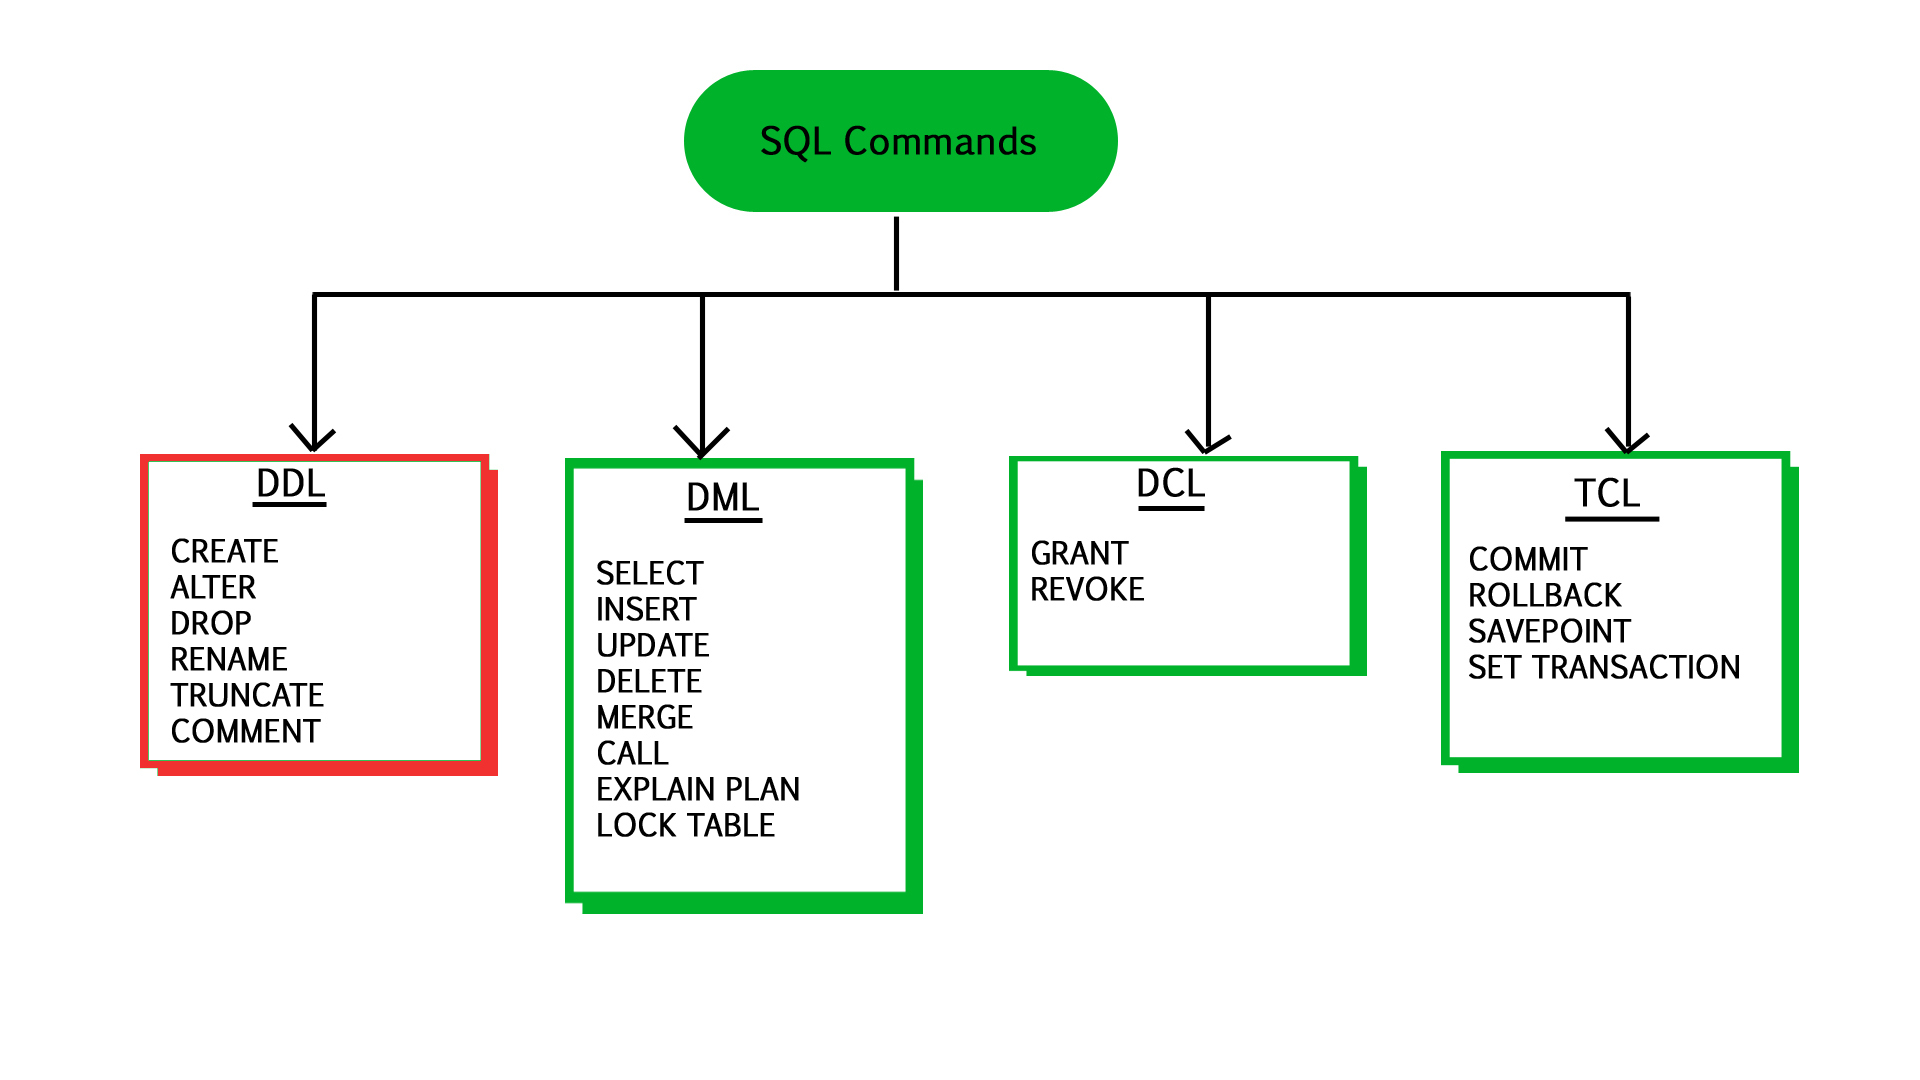
\includegraphics[width=0.75\textwidth]{img//sql-commands-ddl.jpg}
  \label{img:ddl}
\end{figure}

% ############################ CHECK CONSTRAINT ############################
\subsection{CHECK CONSTRAINT}
\label{sec:ddl.check_constraint}
\inputsql{code/ddl/check_constraint.sql}

% ############################ FOREIGN CONSTRAINT ##########################
\subsection{FOREIGN KEY CONSTRAINT}
\label{sec:ddl.foreign_key_constraint}
\inputsql{code/ddl/foreign_key_constraint.sql}

% ############################ PRIMARY CONSTRAINT ##########################
\subsection{PRIMARY KEY CONSTRAINT}
\label{sec:ddl.primary_key_constraint}
\inputsql{code/ddl/primary_key_constraint.sql}

% ############################## MODIFY TABLE ##############################
% \subsection{MODIFY TABLE}
% \label{sec:ddl.modify_table}
% \inputsql{code/ddl/modify_table.sql}

% ############################### RECYCLE_BIN ##############################
% \subsection{RECYCLEBIN}
% \label{sec:dcl.recycle_bin}
% \inputsql{code/ddl/recycle_bin.sql}

% ############################### SEQUENCE ##############################
\subsection{SEQUENCE}
\label{sec:dcl.sequence}
\inputsql{code/ddl/sequence.sql}

% ############################### VIEW ##############################
% \subsection{VIEW}
% \label{sec:dcl.view}
% \inputsql{code/ddl/view.sql}

% ######################## MATERIALIZED VIEW ##############################
\subsection{MATERIALIZED VIEW}
\label{sec:dcl.materialized_view}
\inputsql{code/ddl/materialized_view.sql}

% ######################## EXTERNAL TABLE - CSV##############################
\subsection{EXTERNAL TABLE - CSV}
\label{sec:dcl.external_table}
\inputsql{code/ddl/external_table_csv.sql}
  % ##########################################################################
% ################################### DDL ##################################
% ##########################################################################
\section[DML]{Data-Manipulation-Language}
\label{sec:dml}

\begin{figure}[h]
  \centering
  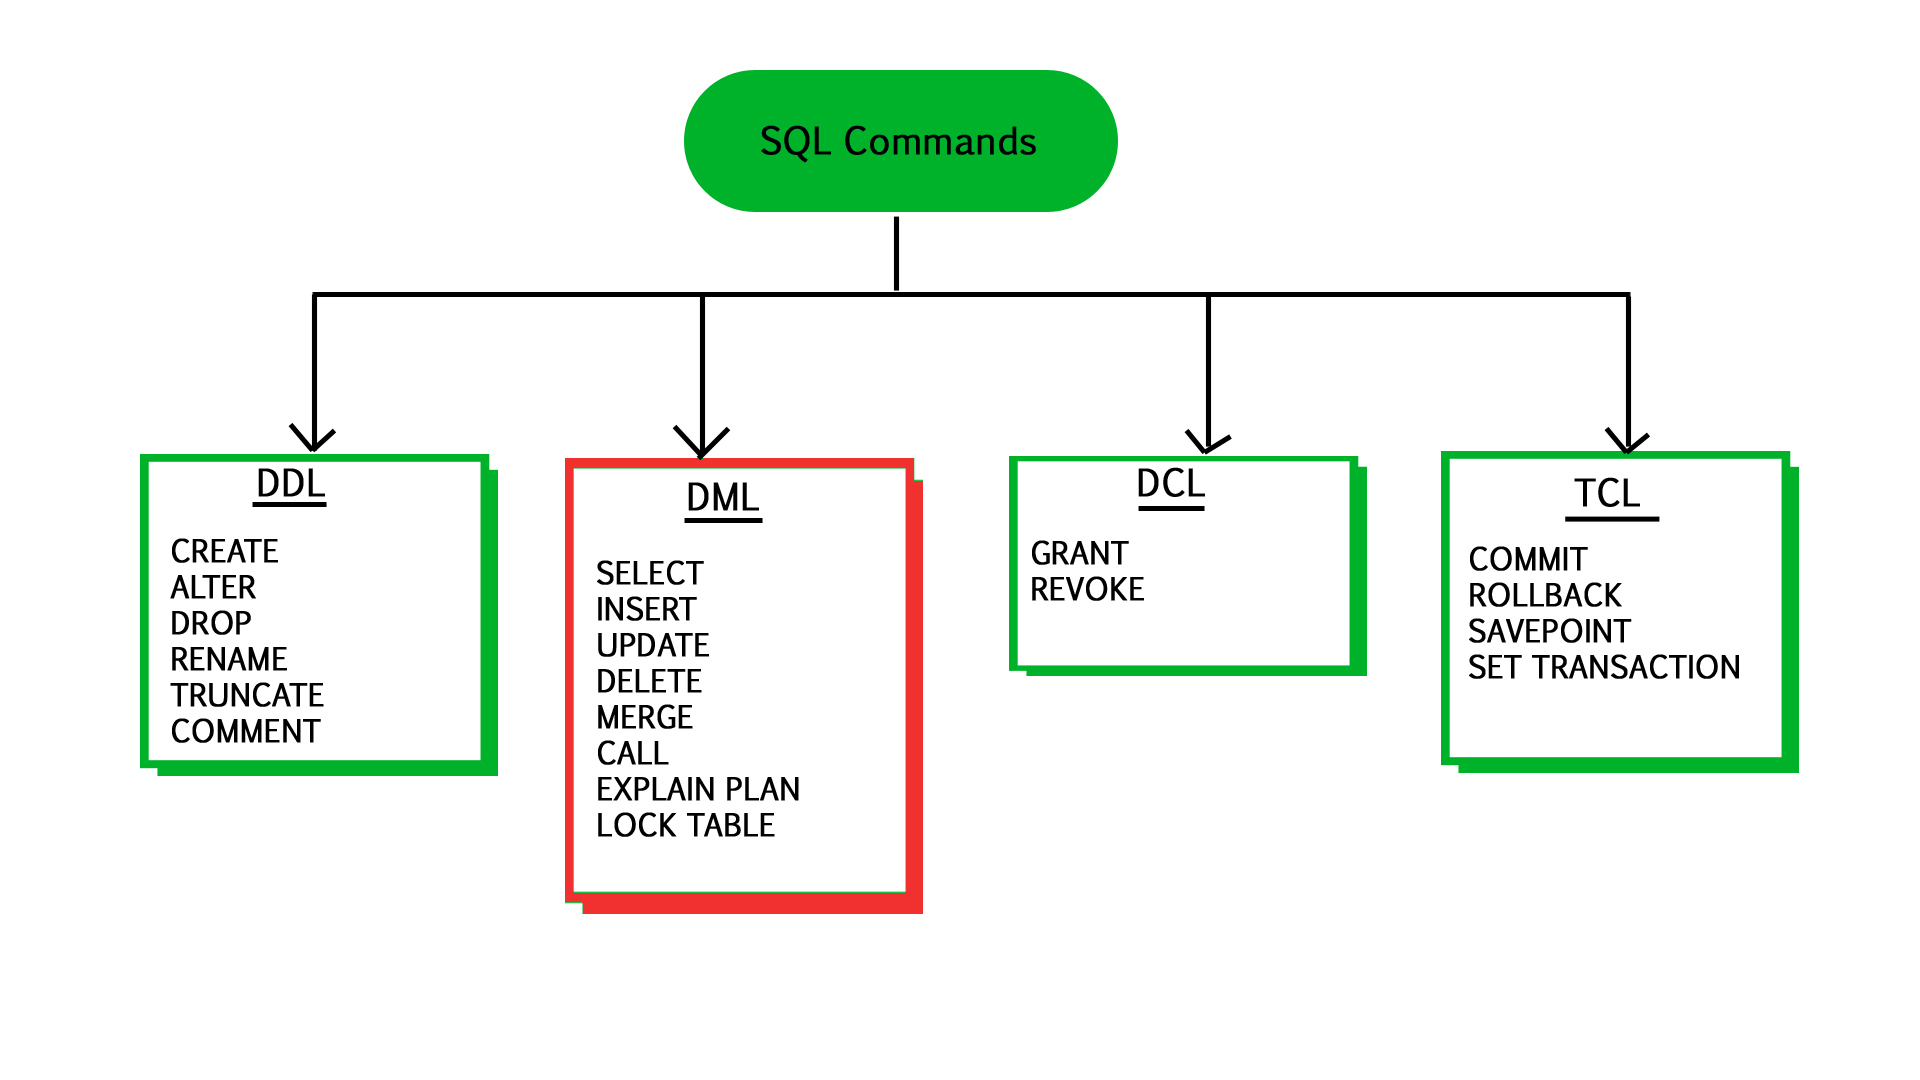
\includegraphics[width=0.75\textwidth]{img//sql-commands-dml.jpg}
  \label{img:dml}
\end{figure}

% ############################### FOR UPDATE ###############################
\subsection{FOR UPDATE}
\label{sec:dml.for_update}
\inputsql{code/dml/for_update.sql}

% ################################ INTERVAL ################################
\subsection{INTERVAL}
\label{sec:dml.interval}
\inputsql{code/dml/interval.sql}

% ################################ TO_CHAR ################################
\subsection{TO\_CHAR}
\label{sec:dml.to_char}
\inputsql{code/dml/to_char.sql}

% ################################ TO_DATE ################################
\subsection{TO\_DATE}
\label{sec:dml.to_date}
\inputsql{code/dml/to_date.sql}
  % ##########################################################################
% ################################### DCL ##################################
% ##########################################################################
\section[DCL]{Data-Controll-Language}
\label{sec:dcl}

\begin{figure}[h]
  \centering
  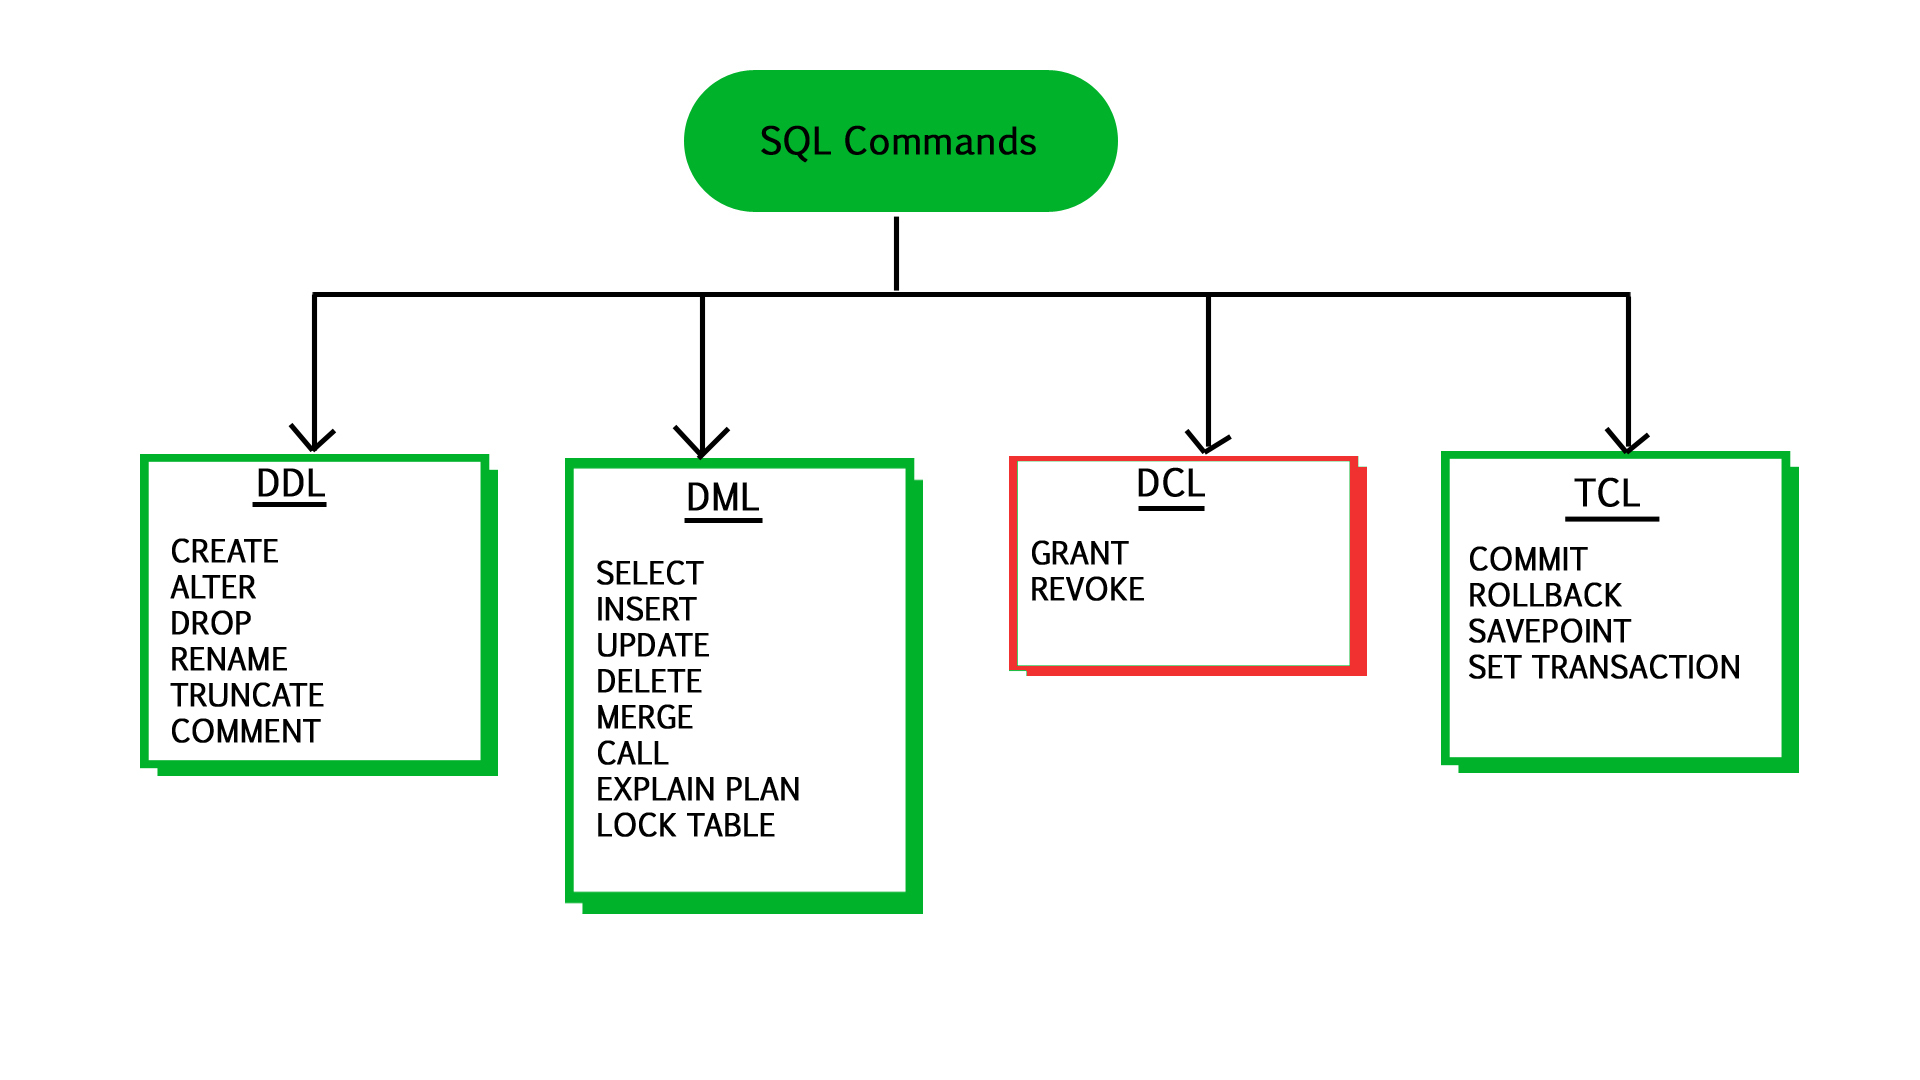
\includegraphics[width=0.75\textwidth]{img//sql-commands-dcl.jpg}
  \label{img:dcl}
\end{figure}

% ################################## GRANT #################################
\subsection{GRANT}
\label{sec:dcl.grant}
\inputsql{code/dcl/grant.sql}

% ################################## REVOKE ################################
\subsection{REVOKE}
\label{sec:dcl.revoke}
\inputsql{code/dcl/revoke.sql}

% ########################### USER_CONS_COLUMNS ############################
\subsection{USER\_CONS\_COLUMNS}
\label{sec:dcl.user_cons_columns}
\inputsql{code/dcl/user_cons_columns.sql}
  % ##########################################################################
% ################################### JSON #################################
% ##########################################################################
\section[JSON]{JavaScript-Object-Notation}
\label{sec:json}

% ############################### JSON_VALUE ###############################
\subsection{JSON\_VALUE}
\label{sec:json.json_value}
\inputsql{code/json/json_value.sql}

% ############################### JSON_TABLE ###############################
\subsection{JSON\_TABLE}
\label{sec:json.jason_table}
\inputsql{code/json/json_table.sql}

% ############################### JSON_QUERY ###############################
\subsection{JSON\_QUERY}
\label{sec:json.jason_query}
\inputsql{code/json/json_query.sql}

% ############################### NESTED PATH ##############################
\subsection{NESTED PATH}
\label{sec:json.nested_path}
\inputsql{code/json/nested_path.sql}

% ############################### JSON EXISTS ##############################
\subsection{JSON EXISTS}
\label{sec:json.json_exists}
\inputsql{code/json/json_exists.sql}


  % Aufzählung aller Bilder
  % \listoffigures
  % \newpage

  % Aufzählung aller Tabellen
  % \listoftables
  % \newpage

  % Glossary
  \printglossaries
  % \newpage

  % Literatur
  % \printbibliography[heading=bibintoc]
\end{document}
